\documentclass[11pt]{article}

% =============================================================================
% WRITING PRINCIPLES FOR THIS PAPER (keep this comment; check against it on
% every edit)
%
% - IMRAD: Introduction, Methods, Results, And Discussion. Related Work is a
%   subsection of the Introduction, not a separate section -- it motivates the
%   problem, it isn't the problem. Compute-budget methodology lives in
%   Methods; the numbers it produces live in Results.
% - Less is more: every sentence must earn its place. If a claim is stated
%   once, do not restate it in the abstract, the section, and the conclusion.
%   Cut adjectives that don't carry information. Prefer one precise number to
%   three qualitative claims.
% - Report what was measured, not what would be interesting if measured.
%   TBD placeholders and "anticipated" tables are not results -- either run
%   the experiment first, or say plainly in Discussion that it's future work,
%   once, and move on.
% - One idea per paragraph, one contribution per bullet, one takeaway per
%   figure/table caption. A caption states what the reader should conclude
%   from the figure, not just what axes it has.
% - State limitations plainly and once, in Discussion. Do not hedge every
%   claim individually throughout the text.
% - Every number in a table must be traceable to a script/config in the repo
%   (this is a lean-research paper, not a position paper) -- prefer citing
%   the exact config path over re-describing the setup in prose. The compute
%   table is generated by scripts/roofline.py and checked by tests/.
% =============================================================================

\usepackage[utf8]{inputenc}
\usepackage[T1]{fontenc}
\usepackage[margin=2.5cm]{geometry}
\usepackage{amsmath,amssymb}
\usepackage{booktabs}
\usepackage{xcolor}
\usepackage{natbib}
\usepackage{tikz}
\usepackage{pgfplots}
\pgfplotsset{compat=1.18}
\usetikzlibrary{arrows.meta,positioning,fit}
\usepackage{algorithm}
\usepackage{algpseudocode}
\usepackage[colorlinks=true,linkcolor=blue!50!black,citecolor=blue!50!black,urlcolor=blue!50!black]{hyperref}
\sloppy

\title{Kairos: A Hybrid Delta/Window-Attention Mixture-of-Experts\\
Denoising Model over a Byte-Level Multimodal Latent Space\\
\large Design, Compute Sizing and a Tiny-Scale Proof of Concept}

\author{Fabien Furfaro\thanks{Code and configurations:
\url{https://github.com/fabienfrfr/Kairos}}}
\date{September 2026}

\begin{document}
\maketitle

\begin{abstract}
Kairos is a proof-of-concept multimodal denoising model that combines
bidirectional gated-DeltaNet linear attention and bidirectional
sliding-window attention over shared projections (LiZAttention2),
block-wise Attention-Residual aggregation, a sparse Mixture-of-Experts
(MoE) feed-forward layer, and a multi-scale byte-level codec, trained with a
uniform-noise denoising objective over a shared byte-level space for text,
image, audio, video, lidar and robot-control streams. We give code-derived
algorithms for each component, including a cross-session recurrent-state
memory gate. We then size a 200M-total/25M-active target with a roofline
model of sparse training: because a microbatch touches nearly every expert,
weight traffic scales with the \emph{total} parameter count, so the
microbatch that makes a sparse model compute-bound is
$N_{\text{total}}/N_{\text{act}}$ times larger than a dense model's (about
1.6k--2.4k tokens on T4, A100 and H100 for our design point, a factor of 8).
Past that threshold the target needs $4.5\times10^{18}$ training FLOPs for
30B tokens; the throughput estimates are upper bounds and none is measured.
Finally, we report a tiny-scale ablation study (1--15M parameters, text
only) whose apparent architectural effects turn out to be
convergence-speed effects on a memorization task: the shared-versus-separate
attention-projection gap closes with more steps or diverse data and reverses
when the suspected mechanism is controlled. No training run at target scale
and no multimodal result is reported.
\end{abstract}

\begin{figure}[ht]
    \centering
    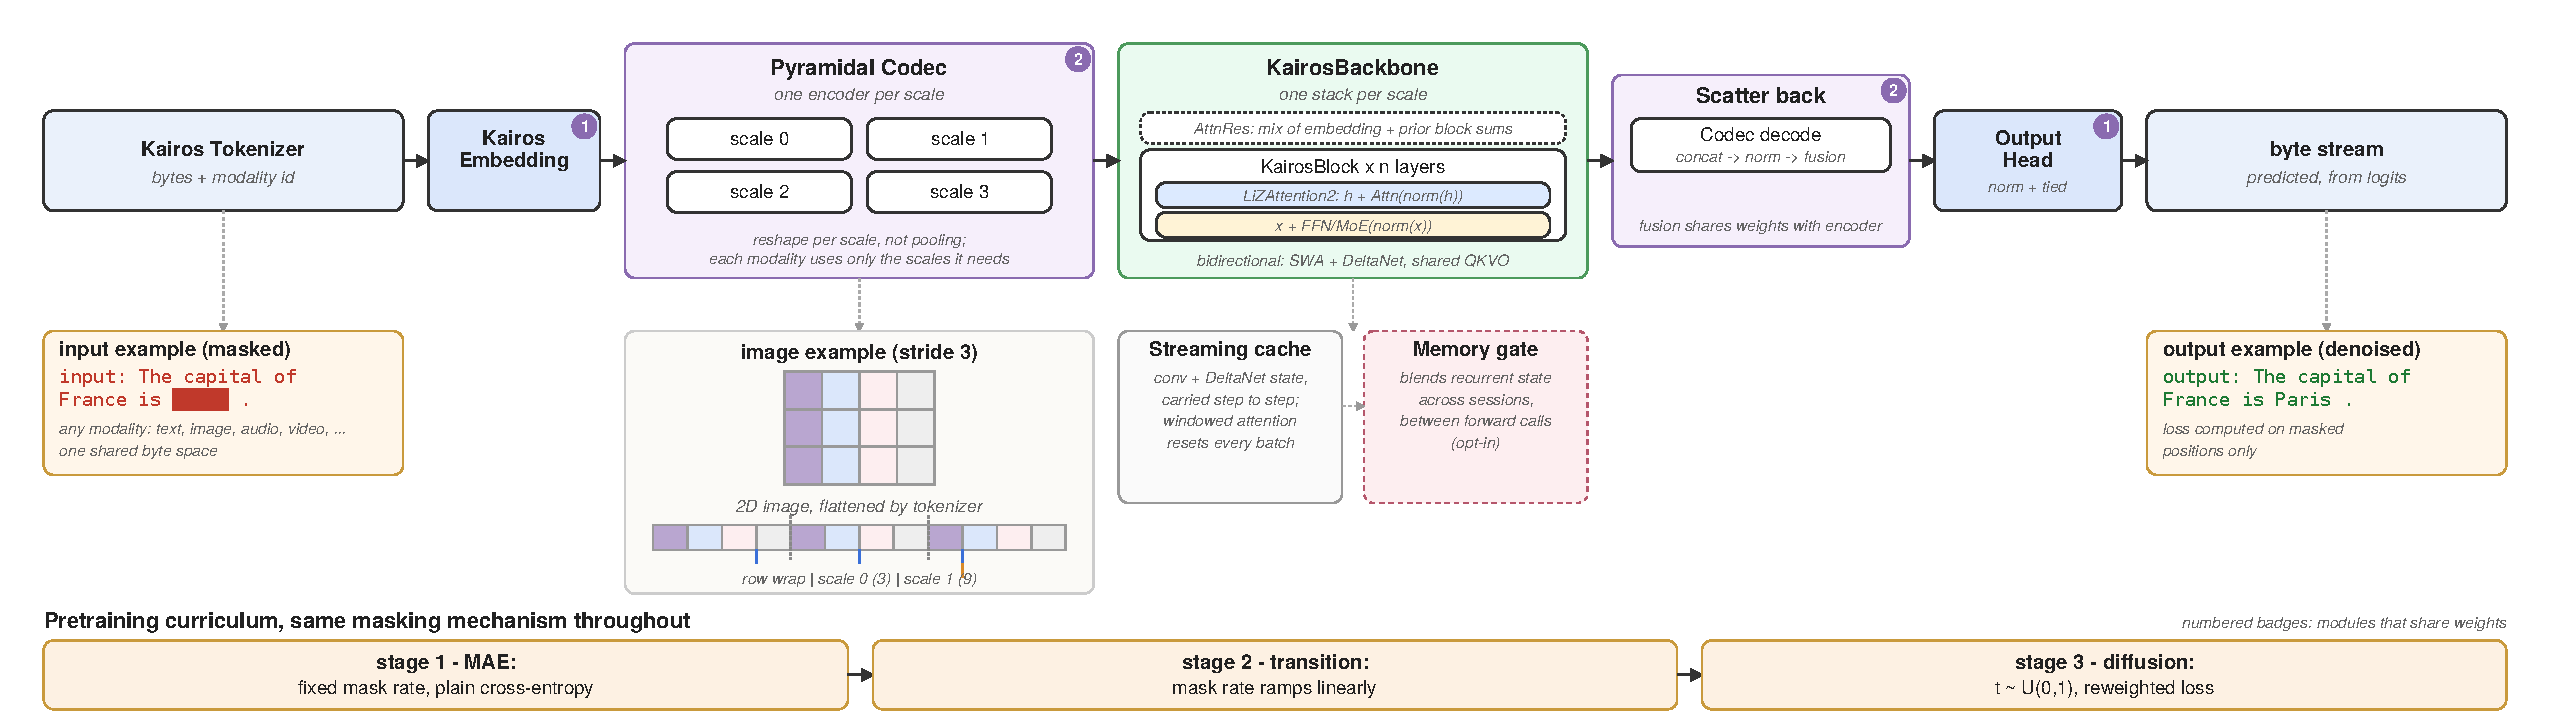
\includegraphics[width=0.95\linewidth]{../architecture/kairos_architecture.pdf}
    \caption{Kairos data and training flow. Byte-level input is embedded, split into
    \texttt{num\_scales} branches by the pyramidal codec, processed by an independent
    DiffusionBackbone per scale (LiZAttention2 in parallel with a routed FFN/MoE, aggregated
    by AttnRes), fused back to $d_{\text{model}}$, and decoded to per-modality logits. Training
    applies the masked-diffusion objective (bottom) on top of this same forward pass; the grey
    box lists the state KairosCache carries across streaming steps.}
    \label{fig:architecture_overview}
\end{figure}

\section{Introduction}

\subsection{Background and problem statement}

Small, edge-deployable language models
(MobileLLM~\citep{liu2024mobilellm}, SmolLM2~\citep{allal2025smollm2},
Gemma~3~\citep{gemma3}) are routinely trained on far more tokens than the
Chinchilla-optimal ratio~\citep{hoffmann2022chinchilla}, on the premise that
inference cost dominates total cost of ownership. That premise says nothing
about training cost when the training hardware is itself constrained, the
setting of this report. Three architectural levers target efficiency in
largely separate literatures: (i) sub-quadratic sequence mixing, through
local windowed attention~\citep{beltagy2020longformer,jiang2023mistral} and
linear state-compressing mixers derived from state-space models
(Mamba~\citep{gu2023mamba}) and the delta
rule~\citep{yang2024deltanet,yang2024gateddeltanet}; (ii) sparse capacity
scaling through MoE
routing~\citep{shazeer2017outrageously,fedus2021switch,dai2024deepseekmoe,deepseekv3};
(iii) non-autoregressive discrete diffusion
training~\citep{austin2021d3pm,lou2023sedd,sahoo2024mdlm,nie2025llada}, which
generalizes masked language modeling~\citep{devlin2018bert}. A fourth,
orthogonal choice removes the tokenizer: byte-level
inputs~\citep{xue2022byt5,yu2023megabyte,pagnoni2024blt} give one vocabulary
that can cover several modalities.

Each lever is usually reported in its own currency (asymptotic sequence
complexity, FLOPs per token, or generation parallelism), and rarely against
the memory-bandwidth limits of the GPUs that motivate combining them.
FLOP-centric accounting of an MoE counts active parameters only, but a
training microbatch routes tokens to many experts, so nearly every expert's
weights are read and its gradients written at every step.
\textbf{Research question:} for a hybrid linear-attention/MoE/denoising model
trained on a single memory-limited GPU, at what microbatch size does sparse
training become compute-bound, and which parameter count, active or total,
is the right one to reduce when it does not?

\subsection{Contributions}

\begin{enumerate}
  \item The Kairos architecture, specified from its implementation:
        PyramidalCodec (Algorithm~\ref{alg:codec}), LiZAttention2
        (Algorithm~\ref{alg:liz}), Block-AttnRes
        (Algorithm~\ref{alg:attnres}), sparse MoE (\S\ref{sec:moe}), a
        cross-session memory gate (Algorithm~\ref{alg:memgate}) and the
        denoising objective with its curriculum
        (Algorithm~\ref{alg:diffusion}), each adapted from a specific prior
        method or, for the codec and the memory gate, combining existing
        ideas.
  \item A roofline model of sparse training (\S\ref{sec:sizing-model}) that
        gives the microbatch threshold above which an MoE is compute-bound,
        applied to a 200M-total/25M-active target
        (\S\ref{sec:sizing-results}); the numbers come from a tested script.
  \item A tiny-scale ablation study (\S\ref{sec:ablations}) with 3-seed
        statistics for codec and attention choices and single-run sweeps for
        seven further factors.
  \item A worked correlation-versus-causation case
        (\S\ref{sec:qkv-sharing}): a clear single-run effect that does not
        survive three controls, and a recommendation to report
        steps-to-threshold rather than loss at a fixed step.
\end{enumerate}

\subsection{Related work}

\paragraph{Efficient attention.} Full self-attention~\citep{vaswani2017attention}
is quadratic in sequence length. The delta
rule~\citep{yang2024deltanet,yang2024gateddeltanet} improves plain linear
attention with an error-correcting state update; Kairos runs it
\emph{bidirectionally} (a forward pass and a time-reversed pass,
concatenated) to match the context a denoising objective needs.
Sliding-window attention~\citep{beltagy2020longformer,jiang2023mistral} is
likewise bidirectional here, with rotary position
embeddings~\citep{su2021roformer}; the code supports grouped-query
attention~\citep{ainslie2023gqa}, which the configurations reported here do
not exercise. Coupling a delta-rule branch and a window-attention branch
through shared projections follows TPTT~\citep{furfaro2025tptt}.

\paragraph{Byte-level, hierarchical and multimodal models.} ByT5 removes the
subword tokenizer~\citep{xue2022byt5}; Kairos' tokenizer subclasses it and
extends it to other modalities. MegaByte models bytes with a global model over
fixed-size patches and a local model inside each
patch~\citep{yu2023megabyte}; the Byte Latent Transformer forms patches
dynamically from next-byte entropy~\citep{pagnoni2024blt}; Hourglass
Transformers shorten and re-expand the sequence inside one
stack~\citep{nawrot2022hourglass}; Perceiver~IO reads arbitrary input arrays,
including raw bytes, through cross-attention into a fixed latent
array~\citep{jaegle2022perceiverio}. Kairos' PyramidalCodec instead keeps
$S$ parallel views of one sequence at geometrically growing patch sizes,
runs a backbone on each, and fuses them after upsampling. We did not perform
a systematic literature search and claim no novelty beyond this combination.

\paragraph{Sparse MoE.} MoE
architectures~\citep{shazeer2017outrageously,fedus2021switch,dai2024deepseekmoe,deepseekv3}
decouple capacity from per-token compute. \texttt{KairosMoE} subclasses
DeepSeek-V3's routed-expert layer~\citep{deepseekv3} (sigmoid routing scores,
shared experts, and load balancing by a per-expert selection bias rather than
an auxiliary loss), and \texttt{KairosFFN}, used when MoE is disabled,
subclasses Qwen2's dense MLP~\citep{qwen2techreport}. Only the expert-weight
initialization is patched, because the upstream implementation used leaves
those weights uninitialized.

\paragraph{Cross-layer residual aggregation.} Block-AttnRes replaces the
fixed, unit-weight residual accumulation standard since
ResNet~\citep{he2015resnet} with the learned, block-windowed softmax
attention over earlier layer outputs of \citet{kimiteam2026attnres}, used
here as published (\S\ref{sec:attnres}).

\paragraph{Discrete diffusion language modeling.} Kairos' corruption is
closest to the uniform-replacement transition of D3PM~\citep{austin2021d3pm}:
corrupted positions are filled with tokens drawn uniformly from the
vocabulary, and the model is not told which positions were corrupted, unlike
the absorbing mask state of MDLM~\citep{sahoo2024mdlm}. The loss is weighted
by $1/p$ in the manner of MDLM, with a clip, and trained with
self-conditioning~\citep{chen2022analogbits} and a three-stage curriculum
(\S\ref{sec:objective}).

\paragraph{Recurrent memory.} Transformer-XL carries hidden states across
segments~\citep{dai2019transformerxl}, Titans learn a test-time
memory~\citep{behrouz2025titans}, and TPTT retrofits such memory into
pretrained transformers~\citep{furfaro2025tptt}. Kairos' gate is simpler: it
seeds the recurrent state of each DeltaNet layer for a new sequence from a
learned blend of states left by earlier sequences (\S\ref{sec:memgate}).

\paragraph{Scaling laws and the cost of sparse training.} Chinchilla is
fitted on dense models from 70M to over 16B
parameters~\citep{hoffmann2022chinchilla}, so applying it to a model with 25M
active parameters is an extrapolation. Joint MoE scaling
laws~\citep{ludziejewski2025moe} add active parameters, tokens and expert
count as variables, and \citet{abnar2025parameters} study the
parameters-versus-FLOPs trade-off at optimal sparsity. These works
parameterize loss rather than step time; we model step time with the
roofline~\citep{williams2009roofline}.

\section{Methods}

\subsection{Three scales, kept apart}

The codebase is used at three scales that this report does not conflate
(Table~\ref{tab:configs}). The \textbf{ablation networks} of
\S\ref{sec:ablations} use the library defaults of
\texttt{configs/ablations/baseline.yaml} (1 layer, dense feed-forward). The
\textbf{PoC configuration} is the default of the project's notebook
(\texttt{notebook/kairos\_pretraining.py}): a $\sim$14--15M-parameter network
with a 7-expert top-1 MoE, used for pipeline sanity checks. The
\textbf{target} is a 200M-total/25M-active design point used in
\S\ref{sec:sizing-model} purely to size a future run; it has never been
instantiated. Because dense parameters (attention, codec, embeddings) are
always active, $N_{\text{act}}=N_{\text{total}}/8+\tfrac78 N_{\text{dense}}$
for $E/k=8$, and 25M is the lower bound reached when all parameters are
routed experts.

\begin{table}[t]
\centering
\small
\begin{tabular}{@{}lp{3.4cm}p{3.9cm}p{2.6cm}@{}}
\toprule
 & Ablation baseline & PoC (notebook) & Target (sizing only) \\
\midrule
$d_{\text{model}}$; heads (head dim) & 64; 4 (16) & 64; 4 (16) & -- \\
Backbone layers & 1 & 4 & -- \\
Codec stride; scales $S$ & 5; 4 & 3; 4 & -- \\
Codec mode & \texttt{conv}, 1 channel per group & \texttt{conv}, 8 channels per group & -- \\
AttnRes block size & 1 & 4 & -- \\
Feed-forward & dense, $I=2048$ & 7 routed ($k=1$) $+$ 1 shared, $I=544$ & 32 routed ($k=4$) \\
Backbone shared across scales & no & yes & -- \\
Memory gate & off & on & -- \\
$N_{\text{total}}$ & 1.98M & $\sim$14--15M & 200M \\
$N_{\text{act}}$ & $N_{\text{total}}$ & $N_{\text{total}}-2.51$M (Eq.~\ref{eq:active}) & 25M \\
Training data & 16 identical sentences, 600 steps & sanity checks & 30B tokens (budget) \\
\bottomrule
\end{tabular}
\caption{The three scales this report distinguishes. Dashes: the target
design point is specified only by its parameter and token budget. The PoC's
$2.51$M is derived from its configuration
($4\times7\times3\times64\times544=2.92$M routed-expert parameters, of which
6/7 are inactive); the instantiated count has not been logged. The ablation
networks are far smaller than the PoC, so ablation findings are not
statements about the PoC.}
\label{tab:configs}
\end{table}

Figure~\ref{fig:architecture} shows the data flow shared by all three.

\begin{figure}[t]
\centering
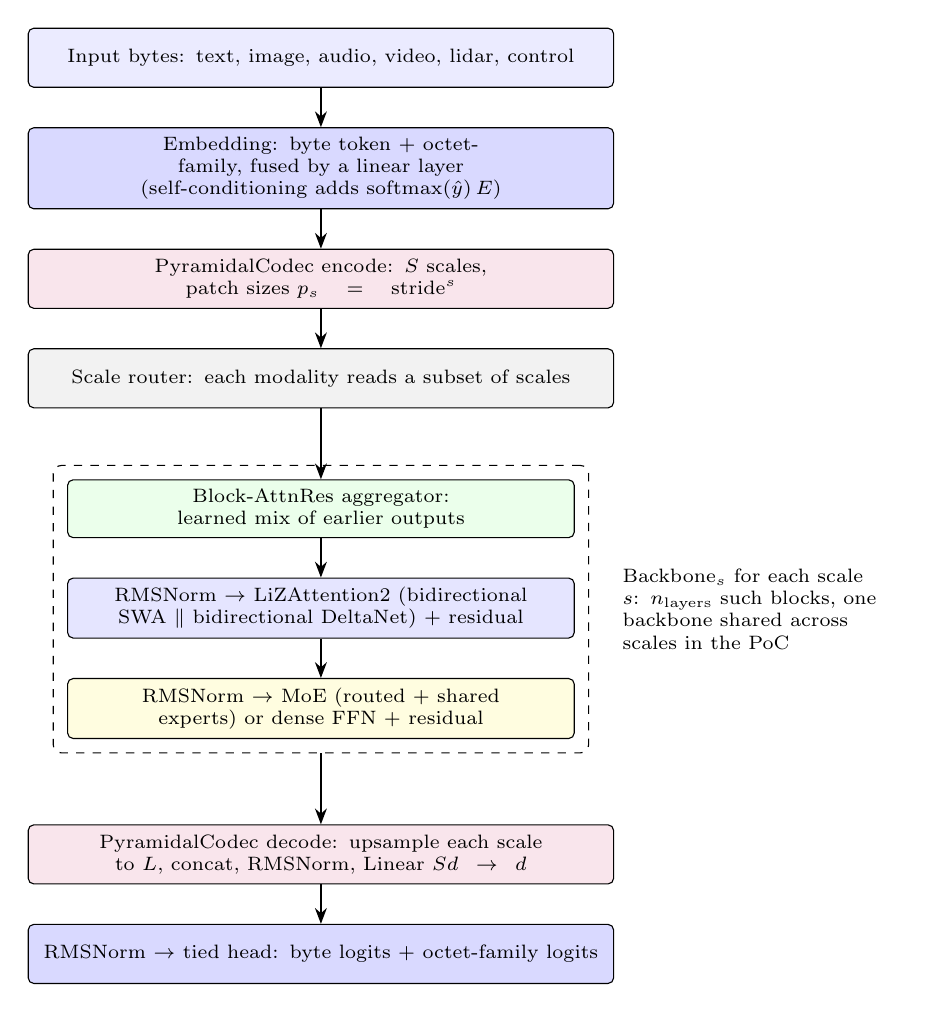
\begin{tikzpicture}[
  font=\small,
  box/.style={draw, rounded corners=2pt, align=center, minimum height=0.75cm, text width=7.2cm, font=\scriptsize},
  inner/.style={draw, rounded corners=2pt, align=center, minimum height=0.65cm, text width=6.2cm, font=\scriptsize, fill=white},
  arr/.style={-{Stealth[length=2mm]}, thick},
  node distance=5mm
]
\node[box, fill=blue!8] (input) {Input bytes: text, image, audio, video, lidar, control};
\node[box, fill=blue!15, below=of input] (embed) {Embedding: byte token $+$ octet-family, fused by a linear layer\\(self-conditioning adds $\mathrm{softmax}(\hat y)\,E$)};
\node[box, fill=purple!10, below=of embed] (enc) {PyramidalCodec encode: $S$ scales, patch sizes $p_s=\text{stride}^s$};
\node[box, fill=gray!10, below=of enc] (route) {Scale router: each modality reads a subset of scales};
\node[inner, fill=green!8, below=9mm of route] (attnres) {Block-AttnRes aggregator: learned mix of earlier outputs};
\node[inner, fill=blue!10, below=of attnres] (liz) {RMSNorm $\to$ LiZAttention2 (bidirectional SWA $\parallel$ bidirectional DeltaNet) $+$ residual};
\node[inner, fill=yellow!12, below=of liz] (moe) {RMSNorm $\to$ MoE (routed $+$ shared experts) or dense FFN $+$ residual};
\node[draw, dashed, rounded corners=3pt, fit=(attnres)(liz)(moe), inner sep=5pt] (blk) {};
\node[right=3mm of blk.east, text width=3.6cm, align=left, font=\scriptsize] {Backbone$_s$ for each scale $s$: $n_{\text{layers}}$ such blocks, one backbone shared across scales in the PoC};
\node[box, fill=purple!10, below=9mm of blk] (dec) {PyramidalCodec decode: upsample each scale to $L$, concat, RMSNorm, Linear $Sd\to d$};
\node[box, fill=blue!15, below=of dec] (head) {RMSNorm $\to$ tied head: byte logits $+$ octet-family logits};
\draw[arr] (input) -- (embed);
\draw[arr] (embed) -- (enc);
\draw[arr] (enc) -- (route);
\draw[arr] (route) -- (attnres);
\draw[arr] (attnres) -- (liz);
\draw[arr] (liz) -- (moe);
\draw[arr] (blk.south) -- (dec);
\draw[arr] (dec) -- (head);
\end{tikzpicture}
\caption{Kairos data flow. The AttnRes aggregator builds the input of each
block; a block is a pre-norm residual pair (attention, feed-forward).
Scales are fused in the codec decoder, after the per-scale backbones.}
\label{fig:architecture}
\end{figure}

\subsection{Byte-level input and PyramidalCodec}

Every modality is serialized to bytes: text as UTF-8, other modalities as
quantized values written as big-endian byte planes (for example a 16-bit audio
sample as a high and a low byte). Each byte is one token, and an auxiliary
\emph{octet-family} id tags which byte plane a token belongs to. Token and
family embeddings are fused by a linear layer; the output head, tied to the
token embedding, predicts both the byte and its family.

The PyramidalCodec builds $S$ parallel views of the sequence with patch sizes
$p_s=\text{stride}^s$ (PoC: stride $3$, $S=4$, so $p=3,9,27,81$). A shared
rank-$r$ bottleneck mixer
($\text{Conv1d}_{d\to r}\to\text{GELU}\to\text{Conv1d}_{r\to d}$,
$r=\max(8,d/4)$, cost $O(rd)$ against $O(d^2)$ for a dense $1{\times}1$
convolution) supplies cross-channel context once; each scale then applies a
grouped convolution with kernel and stride $p_s$ and its own mixer
(Algorithm~\ref{alg:codec}). The group count is the one knob that trades
compute for expressiveness: \texttt{channels\_per\_group}$=1$ (default) is
depthwise and cheapest, and raising it toward $d$ approaches a dense
convolution. \texttt{mode="patch"} replaces the convolution and mixer chain by
one $\text{Linear}(p_s d\to d)$ per scale, decoded with the transposed weight
(tied encode and decode). Each scale runs through its own backbone, or through
one shared backbone (about $75\%$ fewer backbone parameters for $S=4$). A
scale router lets each modality read only a subset of scales (PoC: text
$\to$ scales 1--2, control 1, image 2--3, lidar 2, audio 3, video 3--4,
metadata 4); positions of modalities not routed to a scale bypass its
backbone. Decoding mirrors encoding with grouped transposed convolutions and
per-scale mixers, then concatenates the scales, applies RMSNorm and fuses them
with a linear layer.

\begin{algorithm}[t]
\caption{PyramidalCodec, \texttt{mode="conv"}: encode, per-scale backbone, decode}
\label{alg:codec}
\begin{algorithmic}[1]
\Require $x\in\mathbb{R}^{B\times L\times d}$; patch sizes $p_1,\ldots,p_S$; backbones $f_1,\ldots,f_S$
\State $h\gets\text{Mixer}_{\text{pre}}(x)$ \Comment{shared channel mixing, computed once}
\For{$s=1$ \textbf{to} $S$}
  \State $h_s\gets\text{GroupedConv1d}\big(\text{PadToMultiple}(h,p_s);\ \text{kernel}=\text{stride}=p_s\big)$
  \State $z_s\gets\text{Mixer}_s(h_s)$ \Comment{$\lceil L/p_s\rceil$ positions}
  \State $\tilde z_s\gets f_s(z_s)$ \Comment{active positions only, chosen by the scale router}
  \State $u_s\gets\text{Trim}_L\big(\text{Mixer}'_s(\text{ConvTranspose1d}(\tilde z_s))\big)$
\EndFor
\State \Return $\text{Linear}_{Sd\to d}\big(\text{RMSNorm}(\text{concat}(u_1,\ldots,u_S))\big)$
\end{algorithmic}
\end{algorithm}

\subsection{LiZAttention2: shared-projection bidirectional hybrid attention}
\label{sec:liz}

Each layer runs a bidirectional sliding-window branch (mask $|q-k|\le w$, RoPE)
and a bidirectional gated-DeltaNet branch over the same normalized input. The
DeltaNet branch's Q/K/V and output projections are deleted and replaced by
references to the window branch's, so both mixers read the same linear
projections of $x$ (\texttt{liz2\_share\_qkv=False} restores independent
ones; \S\ref{sec:qkv-sharing}). The DeltaNet branch keeps its own value
expansion (factor 2), depthwise causal convolution, decay and write-strength
gates, output gate, and a merge of its forward and time-reversed passes
(Algorithm~\ref{alg:liz}). The two branch outputs are concatenated,
normalized with RMSNorm~\citep{zhang2019rmsnorm} and projected back to $d$.

\begin{algorithm}[t]
\caption{LiZAttention2 forward (one layer)}
\label{alg:liz}
\begin{algorithmic}[1]
\Require $x\in\mathbb{R}^{B\times L\times d}$; shared projections $W_q,W_k,W_v,W_o$
\State $o^{\text{swa}}\gets W_o\,\text{BidirWindowAttn}\big(\text{RoPE}(W_qx),\text{RoPE}(W_kx),W_vx;\,w\big)$
\For{$\text{dir}\in\{\text{fwd},\text{bwd}\}$}
  \State $x'\gets x$ if fwd, else $\text{flip}(x)$ \Comment{flip along the sequence axis}
  \State $(q,k,v)\gets\text{SiLU}\,\text{DepthwiseCausalConv}\big([W_qx';\,W_kx';\,E_vW_vx']\big)$ \Comment{$E_v$: value expansion}
  \State $\beta\gets\sigma(W_\beta x')$;\quad $g\gets-\exp(A_{\log})\,\text{softplus}(W_ax'+b_{dt})$ \Comment{per head}
  \State $o^{\text{dir}}\gets\text{GatedDeltaRule}(q,k,v;\,g,\beta)\odot\text{SiLU}(W_gx')$ \Comment{$q,k$ L2-normalized}
\EndFor
\State $o^{\Delta}\gets W_o\,W_{\text{lr}}\,\text{RMSNorm}\big([o^{\text{fwd}};\,\text{flip}(o^{\text{bwd}})]\big)$
\State \Return $W_{\text{mix}}\,\text{RMSNorm}\big([o^{\text{swa}};\,o^{\Delta}]\big)$ \Comment{$2d\to d$}
\end{algorithmic}
\end{algorithm}

\subsection{Block-AttnRes aggregation}
\label{sec:attnres}

Instead of the plain residual stream $x_{i+1}=x_i+f_i(x_i)$, each layer's
\emph{input} is a learned, softmax-weighted mix of the embedding, the
finalized block sums of earlier layers, and a running partial sum of the
current block~\citep{kimiteam2026attnres} (Algorithm~\ref{alg:attnres}); the
sublayers of $f_i$ still use ordinary residual connections around their own
input. The weight vector $w$ of each aggregator is initialized to zero, so the
initial mix is uniform. With block size $1$ each earlier layer output is a
separate source, a densely connected pattern~\citep{huang2016densenet} with learned
softmax weights; with block size $n_{\text{layers}}$ the sources reduce to the
embedding and one running sum, and larger sizes change nothing. The PoC uses
block size $4$ over $4$ layers; the ablation networks have one layer, where
the aggregator is a structural no-op.

\begin{algorithm}[t]
\caption{Block-AttnRes backbone forward}
\label{alg:attnres}
\begin{algorithmic}[1]
\Require embedding $x_0$; layers $f_1,\dots,f_L$; block size $S$; learned $w_i\in\mathbb{R}^d$ per aggregator
\State $\text{completed}\gets[\,]$;\ $\text{partial}\gets\text{None}$;\ $\text{count}\gets0$
\For{$i=1,\dots,L$}
  \State $\text{sources}\gets[x_0]\cup\text{completed}\cup(\{\text{partial}\}\text{ if not None})$
  \State $V\gets\text{stack}(\text{sources})$;\quad $K\gets\text{RMSNorm}(V)$
  \State $h\gets\sum_{\text{sources}}\text{softmax}(w_i^{\top}K)\cdot V$ \Comment{softmax over sources}
  \State $x_i\gets f_i(h)$
  \State $\text{partial}\gets x_i$ if partial is None else $\text{partial}+x_i$;\quad $\text{count}\mathrel{+}=1$
  \If{$\text{count}=S$}
    \State $\text{completed}.\text{append}(\text{partial})$;\ $\text{partial}\gets\text{None}$;\ $\text{count}\gets0$
  \EndIf
\EndFor
\State \Return $\text{RMSNorm}(x_L)$
\end{algorithmic}
\end{algorithm}

\subsection{Sparse Mixture-of-Experts}
\label{sec:moe}

Each token is routed to $k$ of $E$ routed experts plus one or more always-on
shared experts. Balance is maintained by nudging a per-expert selection bias
toward equal load (DeepSeek-V3 style, no auxiliary loss by default). The
active-parameter count used throughout is computed directly:
\begin{equation}
N_{\text{act}}=N_{\text{total}}-N_{\text{expert}}+N_{\text{expert}}\frac{k}{E},
\label{eq:active}
\end{equation}
where $N_{\text{expert}}$ sums the parameters under modules whose name
contains \texttt{".experts."}; shared experts, the router, the attention and
DeltaNet path and the codec count as fully active
(\texttt{count\_active\_parameters}).

\subsection{KairosMemoryGate: cross-session recurrent-state memory}
\label{sec:memgate}

With \texttt{use\_memory\_gate=True}, the recurrent state of every DeltaNet
layer of every scale is seeded for a new sequence not from zero but from a
gate over a bank of states left by earlier sequences (the preceding batch's
final state, or an externally supplied bank). One gate module is shared by all
scales and layers. It is a single-head cross-attention over a rank-$r'$
bottleneck, $r'=\max(8,\text{round}(\sqrt{D}/4))$, where $D$ is the flattened
DeltaNet state size ($D=2048$ and $r'=11$ for the PoC). The query is the
projection of the (zero) current state; the keys and values are that same
projection followed by the projected bank, so the gate can attend to the
bank or fall back on the current state (Algorithm~\ref{alg:memgate}). It is
applied to the forward pass only; the time-reversed pass starts from zero.

\begin{algorithm}[t]
\caption{Memory gate, applied per (scale, DeltaNet layer)}
\label{alg:memgate}
\begin{algorithmic}[1]
\Require zero state $s_0\in\mathbb{R}^{B\times D}$; bank $M\in\mathbb{R}^{n\times D}$ of flattened prior states
\If{$n=0$} \State \Return $s_0$ \EndIf
\If{$n=1$} \State \Return $M_1$ broadcast to $B$ rows \EndIf
\State $q\gets\text{Linear}_{D\to r'}(s_0)$;\quad $K\gets[\,q;\ \text{Linear}_{D\to r'}(M)\,]$
\State $o\gets\text{MultiheadAttention}_{h=1}(q,K,K)$
\State \Return $\text{Linear}_{r'\to D}(o)$
\end{algorithmic}
\end{algorithm}

\subsection{Denoising objective and curriculum}
\label{sec:objective}

Given a clean byte sequence $x_0$, each row draws a rate
$p\sim U(\epsilon,p_{\max})$ and a Bernoulli$(p)$ mask over non-prompt,
non-padding positions. Masked positions are replaced by tokens drawn
uniformly from the vocabulary (and random octet-family ids), giving $x_t$; no
mask indicator is provided. The model predicts $x_0$ at the masked positions
with cross-entropy, weighted per token by $\min\!\big(c,\,1+\alpha(1/p-1)\big)$,
a blend between plain cross-entropy ($\alpha=0$) and full $1/p$ weighting
($\alpha=1$) in the manner of MDLM~\citep{sahoo2024mdlm}, clipped at $c$ to
bound the variance from rows with small $p$. With probability $0.5$ per batch,
self-conditioning~\citep{chen2022analogbits} feeds a detached, no-gradient
first prediction back in as an additive embedding, matching its use in
\texttt{generate()}. The default is $\epsilon=10^{-3}$, $c=3$; an
octet-family cross-entropy term with weight $1$ is added when family ids are
present.

\begin{algorithm}[t]
\caption{Denoising training step (\texttt{compute\_loss})}
\label{alg:diffusion}
\begin{algorithmic}[1]
\Require batch $x_0$, prompt lengths, pad mask; schedule values $(p_{\max}^{(t)},\alpha^{(t)})$; clip $c$
\State $p_b\gets\epsilon+(p_{\max}^{(t)}-\epsilon)\,u_b$,\ $u_b\sim U(0,1)$ \Comment{one rate per row}
\State $m\gets\text{Bernoulli}(p_b)$ restricted to non-prompt, non-pad positions
\State $x_t\gets x_0$ with $x_t[m]\gets$ tokens drawn uniformly from the vocabulary
\If{$u<0.5$, $u\sim U(0,1)$} $\hat y\gets\text{stopgrad}(\text{model}(x_t))$; add $\text{softmax}(\hat y)E$ to the embeddings \EndIf
\State $\text{logits}\gets\text{model}(x_t,\ \text{logits\_mask}=m)$ \Comment{project masked positions only}
\State $\ell_i\gets\text{CE}(\text{logits}_i,x_{0,i})\cdot\min\big(c,\,1+\alpha^{(t)}(1/p_{b(i)}-1)\big)$
\State \Return $\text{mean}_i\,\ell_i$ \Comment{$+$ octet-family CE when family ids are present}
\end{algorithmic}
\end{algorithm}

The schedule $(p_{\max}^{(t)},\alpha^{(t)})$ is a pure function of the global
step (\texttt{stage\_mask\_schedule}), so resuming from a checkpoint depends
only on the persisted step count. It is flat at $(0.3,\,0)$ in the MAE stage,
ramps linearly to $(1.0,\,1)$ over the transition stage, then stays flat in
the diffusion stage. The staging was introduced after an informal observation
of optimization instability when sampling the full masking range from a random
initialization; that observation is not quantified here, and no run without
the curriculum is reported.

\subsection{Compute-sizing model}
\label{sec:sizing-model}

Consider one microbatch of $T$ tokens on a GPU with peak dense half-precision
throughput $\pi$ and memory bandwidth $b_s$, whose ridge point is
$\mathcal{I}^\ast=\pi/b_s$~\citep{williams2009roofline}. Training costs
$6N_{\text{act}}T$ FLOPs~\citep{kaplan2020scaling}, ignoring attention-score
FLOPs. Under balanced routing, an expert receives no token with probability
$(1-k/E)^T\approx e^{-Tk/E}$, so for $T\gtrsim5E/k$ (about 40 tokens at
$E=32$, $k=4$; miss probability below $1\%$) essentially every expert is
touched: the forward pass reads $N_{\text{total}}$ weights, not
$N_{\text{act}}$. The backward pass reads them again for activation gradients
and writes the weight gradients, giving $3\beta N_{\text{total}}$ bytes of
weight traffic per microbatch with $\beta=2$ bytes (bf16), independent of $T$.
The arithmetic intensity is therefore
\begin{equation}
\mathcal{I}(T)=\frac{6N_{\text{act}}T}{3\beta N_{\text{total}}}
=\frac{N_{\text{act}}}{N_{\text{total}}}\,T
\quad\text{FLOP/byte},
\label{eq:intensity}
\end{equation}
and the microbatch that reaches the ridge point is
\begin{equation}
T_{\min}=\frac{N_{\text{total}}}{N_{\text{act}}}\,\mathcal{I}^\ast .
\label{eq:tmin}
\end{equation}
Equivalently, each expert must see about $\mathcal{I}^\ast$ tokens per
microbatch, as a dense matrix would. Below $T_{\min}$ the step is bandwidth-bound and
\begin{equation}
\text{throughput}=\frac{T\,b_s}{3\beta N_{\text{total}}}\ \text{tokens/s},
\label{eq:bw}
\end{equation}
which depends on $N_{\text{total}}$ and not on $N_{\text{act}}$. Above
$T_{\min}$ the step is compute-bound at $u\pi/(6N_{\text{act}})$ tokens/s for
a model FLOP utilization $u$, which we assume ($u=25\%$) and do not measure.

Two further terms are estimated separately. An optimizer step reads and writes
fp32 master weights and two Adam moments and reads the gradient, about 30 bytes
per parameter, i.e.\ $30N_{\text{total}}/b_s$ seconds per step, amortized over
the $T_{\text{opt}}$ tokens accumulated per step. The training state occupies
16 bytes per parameter (bf16 weights and gradients, fp32 master weights and
two moments). The model omits activation traffic, DeltaNet states, codec
convolutions, MoE dispatch, kernel-launch overhead and multi-GPU
communication, so it bounds throughput from above.

\subsection{Ablation protocol}
\label{sec:protocol}

All ablations use \texttt{kairos overfit} on the configurations of
\texttt{configs/ablations/} (\texttt{kairos==0.4.1.dev46},
\texttt{torch==2.14.0}), on CPU with eager attention and the PyTorch fallback
DeltaNet path. The data are 16 identical copies of one 440-byte string (the
sentence ``the quick brown fox jumps over the lazy dog'' repeated ten times),
truncated to 128 tokens, i.e.\ about $2.9$ repetitions per sequence; the
63-sentence control uses 63 distinct short sentences. Training uses batch
size 4, 600 steps unless noted, $p_{\max}=0.3$ and no reweighting; the
attention window is the library default $w=128$, which exceeds the 26
positions of the finest scale, so the window branch attends globally. Every
step draws a fresh corruption, and \emph{min.\ loss} is the minimum over the
run of the per-step training loss, an extreme value of a noisy per-batch
quantity. Training and evaluation data coincide, so the study measures
memorization speed, not generalization. Runs are not bit-reproducible even at
a fixed seed: the baseline at seed 0 gave $0.227$ in one run and $0.31$ in
another. Seeds are 0, 1, 2 where stated; standard deviations are sample
standard deviations ($n-1$).

\section{Results}

Two unrelated kinds of result follow, at two scales: \S\ref{sec:sizing-results}
is an analytical sizing of the untrained 200M/25M target, and
\S\ref{sec:ablations} is measured data from the ablation networks. Neither
substitutes for the other.

\subsection{Compute sizing of the target design point}
\label{sec:sizing-results}

The target needs $C=6N_{\text{act}}D=6\times25\text{M}\times30\text{B}=4.5\times10^{18}$
FLOPs. Table~\ref{tab:compute} gives, for three GPUs, the ridge point, the
smallest microbatch that hides the weight traffic of a dense model and of the
sparse target ($N_{\text{total}}/N_{\text{act}}=8$), and the compute-bound
throughput and duration at the assumed $25\%$ utilization
(Figure~\ref{fig:roofline}).

\begin{table}[t]
\centering
\small
\begin{tabular}{lrrrrrrr}
\toprule
GPU & $\pi$ (TFLOPS) & $b_s$ (GB/s) & $\mathcal{I}^\ast$ & $T_{\min}^{\text{dense}}$ & $T_{\min}^{\text{MoE}}$ & tok/s & Days \\
\midrule
T4 & 65 & 320 & 203 & 203 & 1,625 & 108,333 & 3.21 \\
A100 40GB & 312 & 1,555 & 201 & 201 & 1,605 & 520,000 & 0.67 \\
H100 SXM5 & 989 & 3,350 & 295 & 295 & 2,362 & 1,648,333 & 0.21 \\
\bottomrule
\end{tabular}

\caption{Compute-bound sizing of the target ($N_{\text{total}}=200$M,
$N_{\text{act}}=25$M, $D=30$B). $T_{\min}$ is in tokens per microbatch
(Eq.~\ref{eq:tmin}); tok/s and days assume $25\%$ utilization, which is
not measured. Peak dense half-precision throughput $\pi$ and bandwidth $b_s$
are vendor figures~\citep{nvidia2018t4,nvidia2020a100,nvidia2022h100}. The
table is generated by \texttt{scripts/roofline.py}.}
\label{tab:compute}
\end{table}

\begin{figure}[t]
\centering
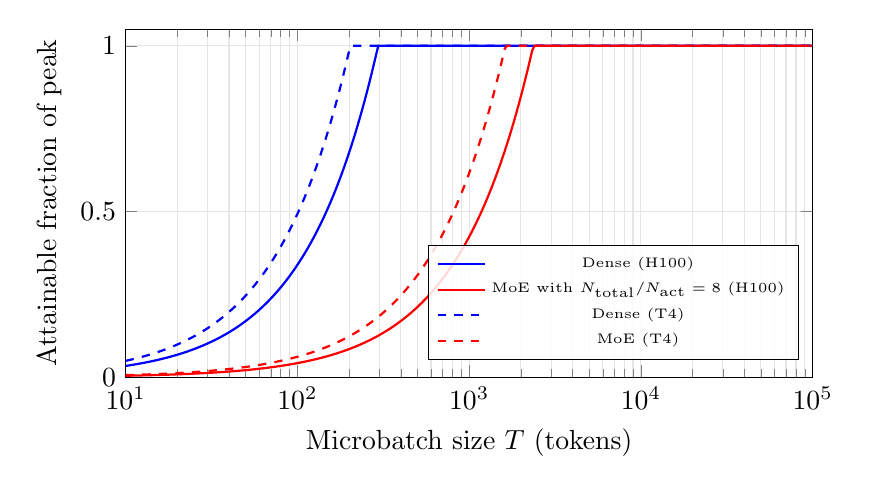
\begin{tikzpicture}
\begin{semilogxaxis}[
  width=0.85\textwidth, height=6cm,
  xlabel={Microbatch size $T$ (tokens)},
  ylabel={Attainable fraction of peak},
  xmin=10, xmax=100000, ymin=0, ymax=1.05,
  legend style={at={(0.98,0.05)}, anchor=south east, font=\tiny, fill=white, fill opacity=0.85, draw opacity=1, text opacity=1},
  grid=both, grid style={gray!20}
]
\addplot[thick, blue, samples=300, domain=10:100000] {min(1, x/295.2)};
\addplot[thick, red, samples=300, domain=10:100000] {min(1, x/(8*295.2))};
\addplot[thick, blue, dashed, samples=300, domain=10:100000] {min(1, x/203.1)};
\addplot[thick, red, dashed, samples=300, domain=10:100000] {min(1, x/(8*203.1))};
\legend{Dense (H100), MoE with $N_{\text{total}}/N_{\text{act}}=8$ (H100), Dense (T4), MoE (T4)}
\end{semilogxaxis}
\end{tikzpicture}
\caption{Model output (Eq.~\ref{eq:intensity}), not a measurement: the
fraction of peak throughput a microbatch can reach. Sparsity moves the
saturation point right by $N_{\text{total}}/N_{\text{act}}=8$.}
\label{fig:roofline}
\end{figure}

A microbatch of about 1.6k tokens (T4, A100) to 2.4k tokens (H100) is enough
for the sparse target to be compute-bound, against about 200--300 tokens for a
dense model of the same size. At $2^{17}$ tokens per optimizer step, the
memory-bound optimizer update adds less than $2.3\%$ to the compute time on
all three GPUs. The 200M-parameter training state takes 3.2~GB and fits a 16~GB
card, leaving the rest for activations, which set the achievable $T$. If
activations or latency cap $T$ below $T_{\min}$, the step time is set by
$N_{\text{total}}$ (Eq.~\ref{eq:bw}); reducing $N_{\text{total}}$ to 50M at
fixed $N_{\text{act}}$ divides $T_{\min}$ by four (about 400--600 tokens).

The target's ratio $D/N_{\text{act}}=1{,}200$ is below that of the dense
Pythia-14M and Pythia-31M, trained on about 300B tokens
($\sim$21{,}000$\times$ and $\sim$9{,}700$\times$ their
parameters)~\citep{biderman2023pythia}. Those models are dense, so they bear
on the plausibility of a high token-to-parameter ratio at small scale, not on
sparse training.

\subsection{Tiny-scale ablation study}
\label{sec:ablations}

Table~\ref{tab:seeds} reports the codec and attention choices under three
seeds, on the setup of \S\ref{sec:protocol}. Codec ranking is identical on
every seed: \texttt{patch} $<$ dense \texttt{conv} $<$ \texttt{conv} with 8
channels per group $<$ depthwise \texttt{conv} (\texttt{liz2}
baseline), from $0.018$ to $0.354$. The hybrid attention beats SWA alone on
every seed ($0.227$, $0.258$, $0.576$ against $0.596$, $0.728$, $0.798$),
although the mean $\pm$ sd ranges overlap. The PoC uses \texttt{conv} with 8
channels per group, a compromise between the depthwise default and the dense
variants.

\begin{table}[t]
\centering
\small
\begin{tabular}{lrrrrr}
\toprule
Configuration & Seed 0 & Seed 1 & Seed 2 & Mean $\pm$ sd & Params \\
\midrule
\texttt{liz2}, depthwise codec (baseline) & 0.227 & 0.258 & 0.576 & $0.354 \pm 0.193$ & 1.98M \\
\texttt{vanilla} (SWA only), depthwise codec & 0.596 & 0.728 & 0.798 & $0.707 \pm 0.103$ & 1.81M \\
\texttt{conv} codec, 8 channels per group & 0.106 & 0.045 & 0.075 & $0.075 \pm 0.031$ & 2.50M \\
\texttt{conv} codec, dense (64 channels per group) & 0.037 & 0.024 & 0.024 & $0.028 \pm 0.007$ & 8.10M \\
\texttt{patch} codec (one \texttt{Linear} per scale) & 0.019 & 0.016 & 0.018 & $0.018 \pm 0.002$ & 4.93M \\
\bottomrule
\end{tabular}
\caption{Minimum training loss after 600 steps, three seeds
(\nolinkurl{docs/experiments/ablations_codec_attention.md}, \S1). Depthwise
saves parameters relative to \texttt{patch} (1.98M against 4.93M) at the cost
of slower memorization; 8 channels per group recovers most of the gap for
about half of \texttt{patch}'s parameters (2.50M against 4.93M). The
\texttt{liz2}-versus-\texttt{vanilla} gap is a convergence-speed effect
(\S\ref{sec:qkv-sharing}).}
\label{tab:seeds}
\end{table}

The seed spread ($\pm0.03$ to $\pm0.19$) sets the noise floor for the
single-run sweeps of Table~\ref{tab:sweeps}, so differences of a few
hundredths there are not readable. Monotone trends are consistent with the
expected direction but confounded with the setup: at 128 tokens a sequence
holds about 2.9 verbatim repetitions of the sentence (1.5 at 64, 5.8 at 256),
so sequence length and the number of codec scales change how many copies are
available for in-context recovery of masked bytes, and the loss reflects
copying as much as memorization. A batch of 16 covers the whole training set.
The attention-block-size result is a saturation effect: sizes at or above the
number of layers give the same computation.

\begin{table}[t]
\centering
\small
\begin{tabular}{p{4.6cm}p{9.6cm}}
\toprule
Factor (base configuration) & Min.\ loss by setting (single run) \\
\midrule
Depth $n_{\text{layers}}$ (\texttt{liz2} baseline) & 1: 0.227;\ 2: 0.843;\ 4: 0.368;\ 8$^{\dagger}$: 1.228 \\
MoE routing, 7 experts & top-1: 0.281;\ top-2: 0.272 \\
Reweighting clip $c$ (diffusion regime, \texttt{conv}, 8 channels per group) & $c=3$: 0.139;\ $c=30$: 0.249 \\
AttnRes block size (4 layers) & 4: 0.386;\ 8: 0.386;\ 16: 0.386 \\
Codec scales $S$ & 2: 0.430;\ 3: 0.308;\ 4: 0.227 \\
Sequence length (tokens) & 64: 1.129;\ 128: 0.227;\ 256: 0.035 \\
Batch size & 1: 0.890;\ 4: 0.227;\ 16 (whole set): 0.032 \\
\bottomrule
\end{tabular}
\caption{Single-run sweeps; read as indicative (\S1 of the log gives the
noise floor). $^{\dagger}$300 steps because of compute budget. The default
$c=10$ is omitted: the log has no per-run record for it. Depth does not help
memorization and top-1 and top-2 routing are indistinguishable at this noise
level.}
\label{tab:sweeps}
\end{table}

\subsubsection{A correlation-versus-causation case: shared versus separate QKV}
\label{sec:qkv-sharing}

Sharing the Q/K/V/O projections between the two attention branches
(\S\ref{sec:liz}) first looked like a clear architectural win: with sharing
disabled, min.\ loss rose from $0.227$--$0.369$ to $0.610$--$0.858$ across
repeated 600-step runs. Three controls were run before accepting this as an
architectural effect (Table~\ref{tab:qkv-sharing}).

\begin{table}[t]
\centering
\small
\begin{tabular}{lrrl}
\toprule
Check & Shared & Separate & Outcome \\
\midrule
600 steps, 16 identical sentences & 0.369 & 0.610 & shared ahead \\
3\,000 steps, same data & 0.0011 & 0.0011 & gap closes \\
63 distinct sentences, 600 steps & 2.269 & 2.285 & gap closes \\
QKV frozen after step 100 & 0.705 & 0.521 & \textbf{gap reverses} \\
\bottomrule
\end{tabular}
\caption{Min.\ loss for shared and separate projections
(\nolinkurl{docs/experiments/ablations_codec_attention.md}, \S7; per-step
curves in \nolinkurl{docs/experiments/liz2_shared_vs_separate_followup_raw.jsonl}).
The advantage was faster early convergence, not higher capacity: with enough
steps or diverse data both variants reach the same floor.}
\label{tab:qkv-sharing}
\end{table}

The same check applies to \texttt{liz2} against \texttt{vanilla}: at
3\,000 steps \texttt{vanilla} reaches $0.0014$, matching \texttt{liz2}'s
$0.0011$. Computing steps-to-threshold from the saved curves shows that the
shared-versus-separate gap is concentrated in the $0.5$--$0.1$ loss range
($+9$ to $+14\%$ steps for separate projections) and vanishes elsewhere,
which a single comparison at a fixed step count would have hidden. A plausible
mechanism is that shared projections receive gradient from both branches at
every step, an effective higher early learning rate. The freezing control is
consistent with it but does not isolate it; a direct test would rescale the
learning rate of the separate variant. The lesson generalizes: a single-run
result on a tiny memorization task is a hypothesis until it survives a
step-budget control, a data-scale control and, where a mechanism is
suspected, a control that isolates it.

\subsubsection{Curriculum and memory gate}

Table~\ref{tab:stages} splits one 600-step run (baseline, seed 0) by
curriculum stage (200 steps each). Losses are not comparable across stages
because the objective changes with $(p_{\max},\alpha)$; the higher tail mean
of the transition stage is consistent with the reweighting ramp raising the
loss scale. This is a single seed, and no run without the curriculum exists.

\begin{table}[t]
\centering
\small
\begin{tabular}{lrr}
\toprule
Stage & First-step loss & Tail-mean loss \\
\midrule
MAE ($p_{\max}=0.3$, $\alpha=0$) & 8.663 & 1.485 \\
Transition (linear ramp) & 1.419 & 2.007 \\
Diffusion ($p_{\max}=1.0$, $\alpha=1$) & 1.873 & 1.555 \\
\bottomrule
\end{tabular}
\caption{Per-stage loss of a single run
(\nolinkurl{docs/experiments/planned_experiments.md}, item 13); the tail
definition is given there.}
\label{tab:stages}
\end{table}

The memory gate was tested through the full training loop for 3 epochs (12
optimizer steps, so absolute losses are not comparable to the rest of the
study): min.\ loss $7.512$ without the gate, $7.453$ with the previous batch's
state only, $7.423$ with a random bank, and final loss $12.927$, $12.893$ and
$9.752$. Twelve steps cannot separate the variants; we draw no conclusion.

\section{Discussion}

\paragraph{Compute sizing.} Under the model of \S\ref{sec:sizing-model}, a
sparse model trains at compute-bound speed only when its microbatch exceeds
$N_{\text{total}}/N_{\text{act}}$ times the dense threshold; below that,
throughput is set by $N_{\text{total}}$, not by the active parameters that
FLOP-centric accounting counts. Sparsity is therefore not free on
memory-limited hardware: $E/k$ multiplies the microbatch needed for
compute-bound execution, and activation memory grows with the microbatch.
Whether a 16~GB card holds a 2.4k-token microbatch of this architecture is an
empirical question this report does not answer.

\paragraph{Ablations.} The only architectural comparisons tested at a longer
horizon (\texttt{liz2} against \texttt{vanilla}, shared against separate
projections) show no capacity difference. The codec ranking of
Table~\ref{tab:seeds} is stable across seeds but has not been tested at longer
horizons or on diverse data, and should be read as a memorization-speed
ranking.

\subsection{Limitations}

The target-scale analysis is a sizing model for a run that has not been
performed: throughput is an upper bound at an assumed utilization, it assumes
balanced routing and counts weight and optimizer traffic only, and the
Chinchilla comparison is an extrapolation. The ablation study memorizes one
sentence in 16 copies on text only, with a window branch that attends
globally, on CPU, with runs that are not bit-reproducible; its metric is a
minimum over noisy per-step losses. Only Table~\ref{tab:seeds} and
\S\ref{sec:qkv-sharing} carry multi-seed or multi-control statistics; the
other sweeps are single-run. Parameter counts of the ablation rows in
Table~\ref{tab:seeds} other than the baseline are carried over from earlier
logs. The PoC's active-parameter count has not been logged from an
instantiated model. No dense baseline is compared, so nothing here supports a
claim of superiority; the multimodal, curriculum and memory-gate components
have no supporting result yet.

\subsection{Future work}

Four experiments would turn this report's hypotheses into findings: (i) a
measured tokens/s against microbatch size for the 200M/25M and a 50M/25M
variant on a T4 and an A100/H100, which tests Eqs.~\ref{eq:tmin}
and~\ref{eq:bw} directly; (ii) 3-seed, steps-to-threshold reruns of the
single-run sweeps on diverse data; (iii) per-modality loss on real multimodal
data; (iv) a run without the curriculum.

\section{Conclusion}

Kairos is a proof of concept of 1--15M parameters that runs a hybrid
bidirectional DeltaNet/window-attention, MoE, denoising architecture end to
end over a byte-level multimodal space, with a separate 200M/25M design point
used only to size a future run. For that design point, sparse training is
compute-bound once each expert sees about a ridge point's worth of tokens per
microbatch, roughly 1.6k--2.4k tokens; the ablation study's main result is
methodological, since its clearest architectural effect was a convergence-speed
artifact.

\section*{Code and reproducibility}

Code, configurations and logs are in the repository. Ablation configurations
are in \texttt{configs/ablations/}; a run is
\texttt{kairos overfit configs/ablations/<name>.yaml --steps 600 --mask-p-max 0.3
--no-mask-reweight --seed <0|1|2>}. The compute table is produced by
\texttt{python scripts/roofline.py > docs/paper/tables/compute.tex} and checked
by \texttt{tests/test\_roofline.py} and \texttt{tests/test\_paper.py}.

\bibliographystyle{plainnat}
\bibliography{kairos_references}

\end{document}
